\section{Tạo bảng và dữ liệu mẫu}
\subsection{Sơ đồ mô hình dữ liệu quan hệ}
\begin{figure}[H]
    \centering
    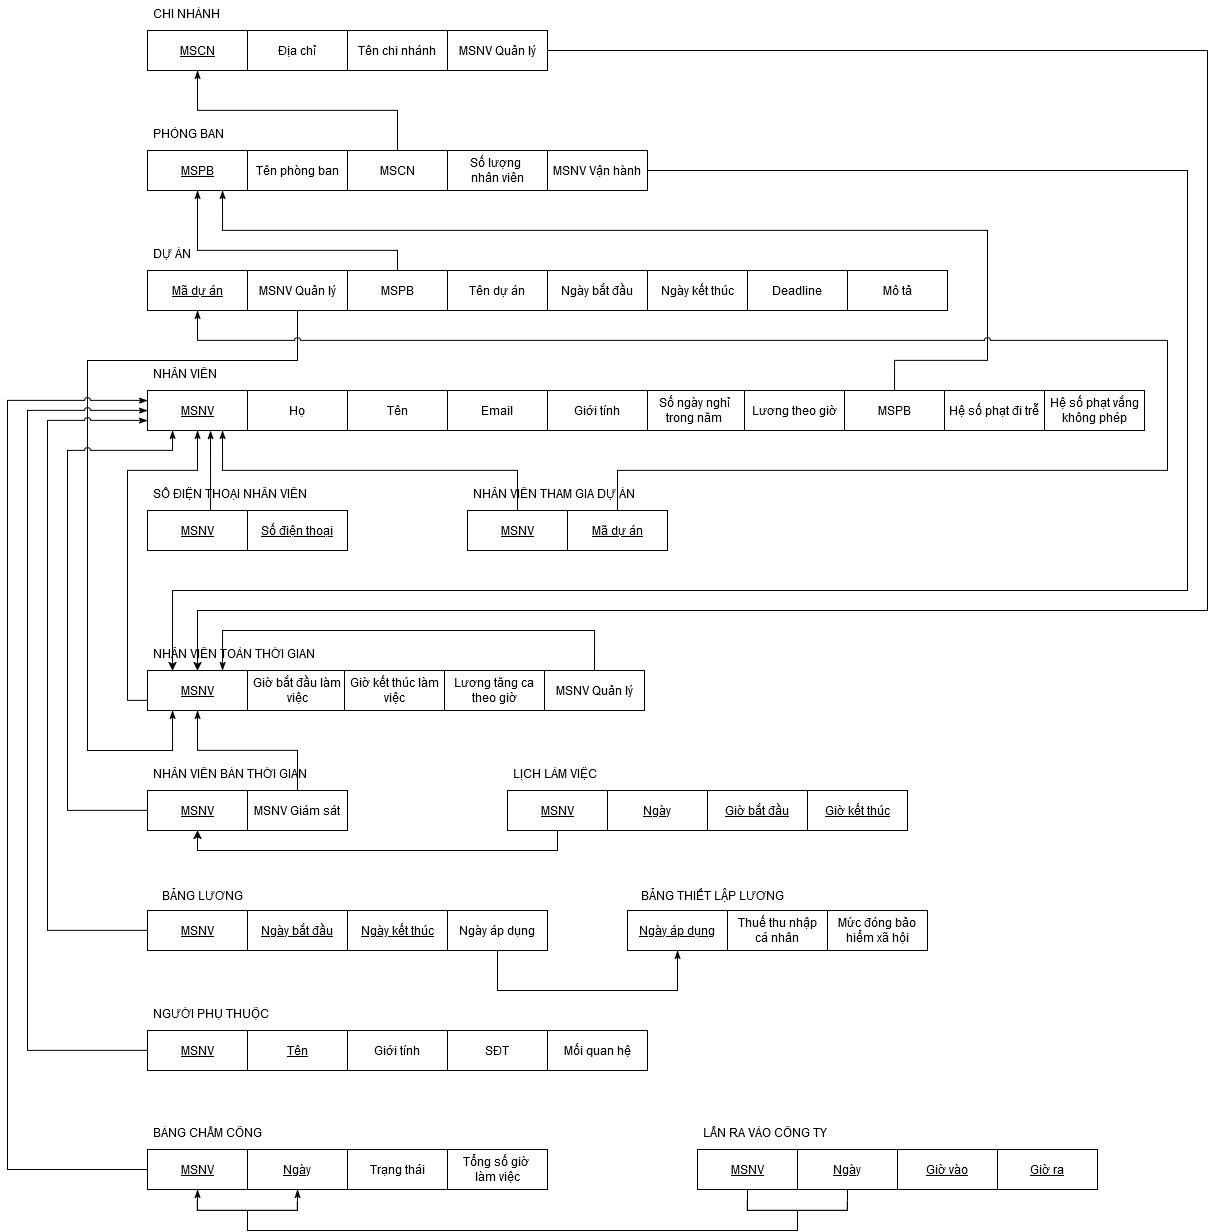
\includegraphics[width=\linewidth]{content/images/relational-mapping.jpg}
    \caption{Mô hình dữ liệu quan hệ của hệ thống}
    \label{fig:relational-mapping}
\end{figure}

\newpage
\subsection{Hiện thực các bảng và tạo dữ liệu mẫu}
\subsubsection{Bảng ChiNhanh}
\begin{itemize}
    \item [--] Câu lệnh tạo bảng
   \begin{minted}{mysql}
CREATE TABLE ChiNhanh (
    MaChiNhanh CHAR(4) PRIMARY KEY,
    TenChiNhanh NVARCHAR(100) NOT NULL,
    DiaChi NVARCHAR(200) NOT NULL,
    MSNV_QuanLy CHAR(6)
);
-- Sau khi đã import đủ data thì thêm thuộc tính khóa ngoại
ALTER TABLE chinhanh 
    ADD FOREIGN KEY (MSNV_QuanLy) REFERENCES nhanvientoanthoigian(MaNV);
    \end{minted}
    \newpage
    \item [--] Câu lệnh ràng buộc
    \begin{minted}{mysql}
-- Trigger để kiểm tra định dạng của dữ liệu trước khi thực hiện INSERT
DELIMITER //
CREATE TRIGGER IF NOT EXISTS checkChiNhanhFormat
BEFORE INSERT on ChiNhanh
FOR EACH ROW
BEGIN 
    IF NEW.MaChiNhanh NOT REGEXP '^CN[0-9]{2}$' THEN
        SIGNAL SQLSTATE '45000'
        SET MESSAGE_TEXT = 'Mã chi nhánh phải ở định dạng CNxx, với xx là hai chữ số bất kỳ';
    END IF;

    IF NEW.TenChiNhanh NOT REGEXP '^[[:alnum:][:space:].,\\-]*$' THEN 
        SIGNAL SQLSTATE '45000'
        SET MESSAGE_TEXT = 'Tên chi nhánh không được chứa ký tự đặc biệt';
    END IF;

    IF NEW.DiaChi NOT REGEXP '^[[:alnum:][:space:].,\\-]*$' THEN 
        SIGNAL SQLSTATE '45000'
        SET MESSAGE_TEXT = 'Địa chỉ không được chứa ký tự đặc biệt';
    END IF;

    IF (NEW.MSNV_QuanLy IS NOT NULL) AND (NOT EXISTS (SELECT 1 from nhanvien WHERE nhanvien.`MaNV`=NEW.MSNV_QuanLy)) THEN
        SIGNAL SQLSTATE '45000'
        SET MESSAGE_TEXT = 'Mã số nhân viên quản lý không tồn tại';
    END IF;
END //
DELIMITER ;
    \end{minted}
    \newpage
    \item [--] Câu lệnh thêm dữ liệu
   \begin{minted}{mysql}
INSERT INTO ChiNhanh (MaChiNhanh, TenChiNhanh, DiaChi) 
VALUES 
    ('CN01', 'Chi nhánh Cần Thơ', '321 Đường Cần Thơ, Cần Thơ'),
    ('CN02', 'Chi nhánh Hải Phòng', '654 Đường Hải Phòng, Hải Phòng'),
    ('CN03', 'Chi nhánh Huế', '987 Đường Huế, Huế'),
    ('CN04', 'Chi nhánh Vinh', '234 Đường Vinh, Nghệ An');
    
-- Cập nhật thuộc tính MSNV_QuanLy sau khi đã thêm dữ liệu ở bảng NhanVienToanThoiGian
UPDATE chinhanh SET `MSNV_QuanLy` = 'NV3058' WHERE `MaChiNhanh` = 'CN01';
UPDATE chinhanh SET `MSNV_QuanLy` = 'NV9225' WHERE `MaChiNhanh` = 'CN02';
UPDATE chinhanh SET `MSNV_QuanLy` = 'NV9433' WHERE `MaChiNhanh` = 'CN03';
UPDATE chinhanh SET `MSNV_QuanLy` = 'NV1452' WHERE `MaChiNhanh` = 'CN04';
    \end{minted}
    \item [--] Kết quả dữ liệu của bảng
    \begin{figure}[H]
        \centering
        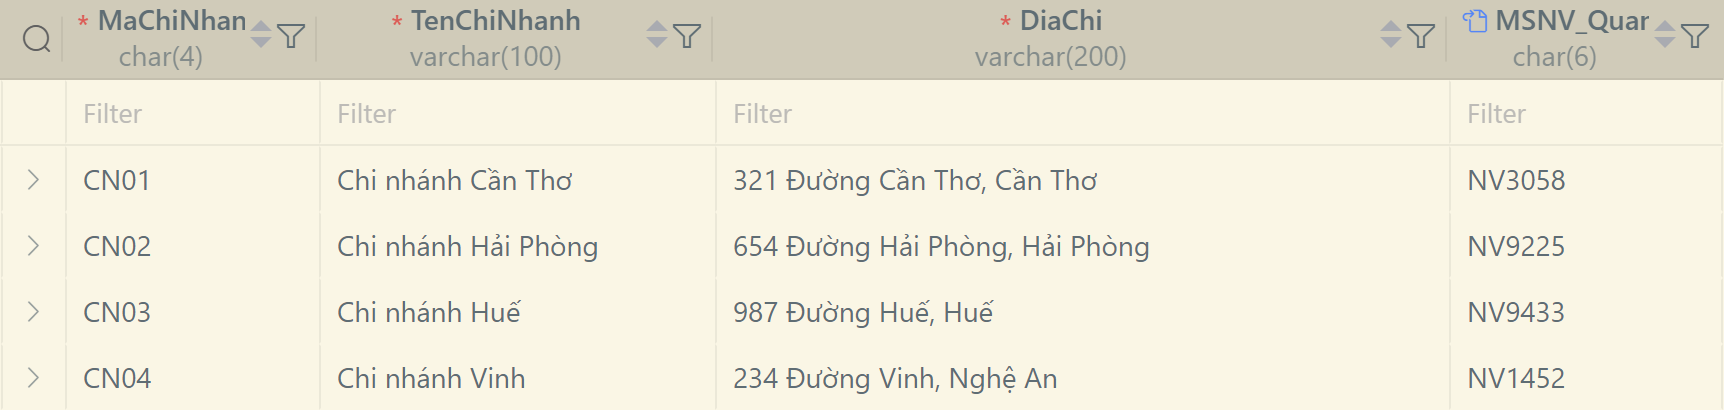
\includegraphics[width=1\linewidth]{content/images/data_chinhanh.png}
        \caption{Dữ liệu bảng ChiNhanh}
        \label{fig:data_chinhanh}
    \end{figure}
\end{itemize}
\newpage
\subsubsection{Bảng PhongBan}
\begin{itemize}
    \item [--] Câu lệnh tạo bảng
   \begin{minted}{mysql}
CREATE TABLE PhongBan (
    MaPhongBan CHAR(6) PRIMARY KEY,
    TenPhongBan NVARCHAR(100) NOT NULL,
    MaChiNhanh CHAR(4) NOT NULL,
    SoLuongNhanVien INT DEFAULT 0,
    MSNV_VanHanh CHAR(6),
    FOREIGN KEY (MaChiNhanh) REFERENCES ChiNhanh(MaChiNhanh)
);
-- Thêm thuộc tính khóa ngoại sau khi import đủ thông tin ở bảng khác
ALTER TABLE phongban
    ADD FOREIGN KEY (MSNV_VanHanh) REFERENCES nhanvientoanthoigian(MaNV);
    \end{minted}
    \newpage
    \item [--] Câu lệnh ràng buộc
    \begin{minted}{mysql}
CREATE TRIGGER IF NOT EXISTS checkPhongBanFormat
BEFORE INSERT on PhongBan
FOR EACH ROW
BEGIN 
    IF NEW.MaPhongBan NOT REGEXP '^PB[0-9]{4}$' THEN
        SIGNAL SQLSTATE '45000'
        SET MESSAGE_TEXT = 'Mã phòng ban phải ở định dạng PBxxxx, với xxxx là bốn chữ số bất kỳ';
    END IF;

    IF NEW.TenPhongBan NOT REGEXP '^[[:alnum:][:space:].,\\-]*$' THEN 
        SIGNAL SQLSTATE '45000'
        SET MESSAGE_TEXT = 'Tên phòng ban không được chứa ký tự đặc biệt';
    END IF;

    IF NOT EXISTS (SELECT 1 FROM chinhanh where chinhanh.`MaChiNhanh`=NEW.MaChiNhanh) THEN 
        SIGNAL SQLSTATE '45000'
        SET MESSAGE_TEXT = 'Mã chi nhánh không tồn tại';
    END IF;

    IF (NEW.MSNV_VanHanh IS NOT NULL) AND (NOT EXISTS (SELECT 1 from nhanvien WHERE nhanvien.`MaNV`=NEW.MSNV_VanHanh)) THEN
        SIGNAL SQLSTATE '45000'
        SET MESSAGE_TEXT = 'Mã số nhân viên vận hành không tồn tại';
    END IF;
END //
    \end{minted}
    \newpage
    \item [--] Câu lệnh thêm dữ liệu
   \begin{minted}{mysql}
INSERT INTO PhongBan (MaPhongBan, TenPhongBan, MaChiNhanh)
VALUES
    ('PB0101', 'Phòng Kế toán', 'CN01'),
    ('PB0102', 'Phòng Nhân sự', 'CN01'),
    ('PB0103', 'Phòng Kỹ thuật', 'CN01'),
    ('PB0104', 'Phòng IT', 'CN01'),
    ('PB0105', 'Phòng Marketing', 'CN01'),
    ...;

-- Cập nhật thuộc tính MSNV_VanHanh sau khi đã thêm dữ liệu ở bảng NhanVienToanThoiGian
UPDATE phongban SET `MSNV_VanHanh` = 'NV8120' WHERE `MaPhongBan` = 'PB0101';
UPDATE phongban SET `MSNV_VanHanh` = 'NV6786' WHERE `MaPhongBan` = 'PB0102';
UPDATE phongban SET `MSNV_VanHanh` = 'NV7040' WHERE `MaPhongBan` = 'PB0103';
UPDATE phongban SET `MSNV_VanHanh` = 'NV4036' WHERE `MaPhongBan` = 'PB0104';
UPDATE phongban SET `MSNV_VanHanh` = 'NV1404' WHERE `MaPhongBan` = 'PB0105';
...
    \end{minted}
    \item [--] Kết quả dữ liệu của bảng
    \begin{figure}[H]
        \centering
        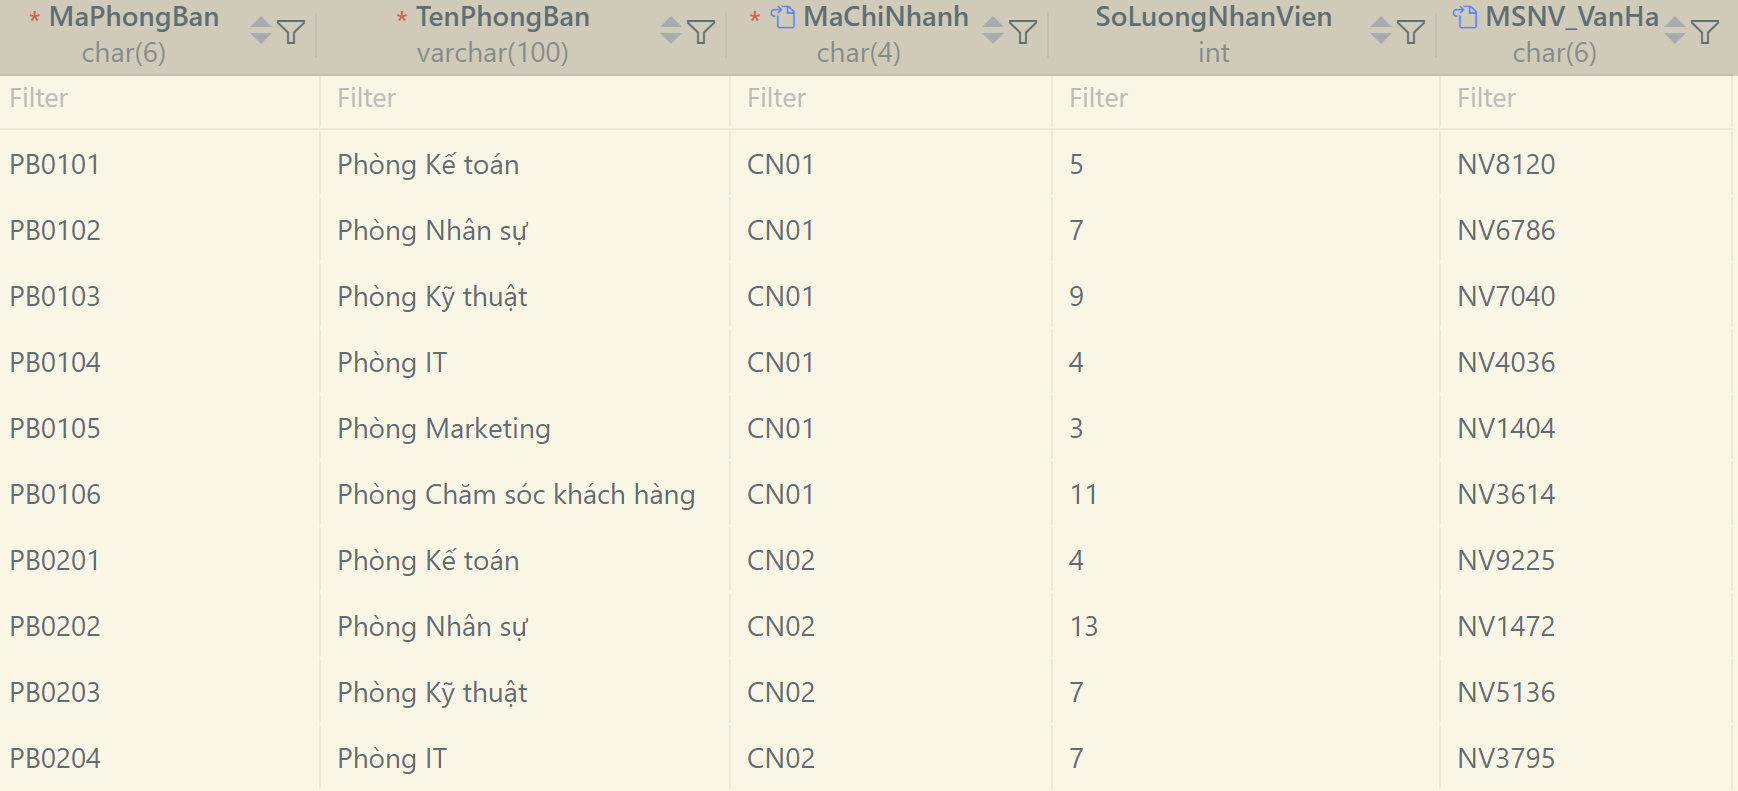
\includegraphics[width=\linewidth]{content/images/data_phongban.png}
        \caption{Dữ liệu bảng PhongBan}
        \label{fig:data_phongban}
    \end{figure}
\end{itemize}
\newpage
\subsubsection{Bảng NhanVien}
\begin{itemize}
    \item [--] Câu lệnh tạo bảng
    \begin{minted}{mysql}
CREATE TABLE NhanVien (
    MaNV CHAR(6) PRIMARY KEY,
    Ho NVARCHAR(10) NOT NULL,
    TenLot NVARCHAR(10),
    Ten NVARCHAR(10) NOT NULL,
    GioiTinh ENUM('Nam', 'Nữ', 'Khác') NOT NULL,
    Email VARCHAR(100) NOT NULL UNIQUE,
    HeSoPhatDiTre DECIMAL(5, 2) DEFAULT 1,
    HeSoPhatVangKhongPhep DECIMAL(5, 2) DEFAULT 1,
    SoNgayNghi INT DEFAULT 12,
    LuongTheoGio DECIMAL(10, 2) NOT NULL,
    MaPhongBan CHAR(6),
    FOREIGN KEY (MaPhongBan) REFERENCES PhongBan(MaPhongBan)
);
    \end{minted}
    \newpage
    \item [--] Câu lệnh ràng buộc
    \begin{minted}{mysql}
DELIMITER //
CREATE TRIGGER IF NOT EXISTS checkNhanVienFormat
BEFORE INSERT ON nhanvien
FOR EACH ROW
BEGIN
    IF NEW.MaNV NOT REGEXP '^NV[0-9]{4}$' THEN
        SIGNAL SQLSTATE '45000' 
        SET MESSAGE_TEXT = 'Mã nhân viên phải có định dạng NVxxxx, với 4 chữ số đằng sau';
    END IF;

    IF NEW.Ho NOT REGEXP '^[[:alnum:]]*$' THEN 
        SIGNAL SQLSTATE '45000'
        SET MESSAGE_TEXT = 'Họ chỉ gồm một từ và không được chứa ký tự đặc biệt';
    END IF;

    IF NEW.TenLot NOT REGEXP '^[[:alnum:][:space:]]*$' THEN 
        SIGNAL SQLSTATE '45000'
        SET MESSAGE_TEXT = 'Tên lót không được chứa ký tự đặc biệt';
    END IF;

    IF NEW.Ten NOT REGEXP '^[[:alnum:]]*$' THEN 
        SIGNAL SQLSTATE '45000'
        SET MESSAGE_TEXT = 'Tên chỉ gồm một từ và không được chứa ký tự đặc biệt';
    END IF;

    IF NEW.Email NOT REGEXP '^[a-zA-Z0-9._%+-]+@[a-zA-Z0-9.-]+\.[a-zA-Z]{2,}$' THEN
        SIGNAL SQLSTATE '45000' 
        SET MESSAGE_TEXT = 'Email không đúng định dạng.';
    END IF;
    ...
    IF EXISTS (SELECT 1 FROM nhanvien WHERE nhanvien.Email = NEW.Email) THEN 
        SIGNAL SQLSTATE '45000' SET MESSAGE_TEXT = 'Email nhân viên đã tồn tại';
    END IF;
END//
DELIMITER ;
    \end{minted}
    \newpage
    \item [--] Câu lệnh thêm dữ liệu
   \begin{minted}{mysql}
INSERT INTO NhanVien (MaNV, Ho, TenLot, Ten, GioiTinh, Email, LuongTheoGio, MaPhongBan)
VALUES
    ('NV8058', 'Văn', 'Phú', 'Ân', 'Nam', 'vanphuan@gmail.com', 90000, 'PB0106'),
    ('NV9750', 'Kim', 'Hải', 'Sơn', 'Nam', 'kimhaison@gmail.com', 60000, 'PB0205'),
    ('NV2034', 'Thi', 'Dũng', 'Trí', 'Nữ', 'thidungtri@gmail.com', 80000, 'PB0301'),
    ('NV2790', 'Tô', 'Đức', 'Duy', 'Nam', 'toducduy@gmail.com', 25000, 'PB0401'),
    ('NV1452', 'Lục', 'Thuận', 'Thành', 'Khác', 'lucthuanthanh@gmail.com', 100000, 'PB0402'),
    ('NV9714', 'Sái', 'Thế', 'An', 'Nữ', 'saithean@gmail.com', 60000, 'PB0204'),
    ('NV9858', 'Nguyễn', 'Việt', 'Khôi', 'Khác', 'nguyenvietkhoi@gmail.com', 50000, 'PB0106'),
    ('NV7733', 'Đoàn', 'Hữu', 'Trung', 'Nữ', 'doanhuutrung@gmail.com', 25000, 'PB0101'),
    ('NV9240', 'Phạm', 'Anh', 'Tài', 'Khác', 'phamanhtai@gmail.com', 40000, 'PB0206')
    ...;
    \end{minted}
    \item [--] Kết quả dữ liệu của bảng
    \begin{figure}[H]
        \centering
        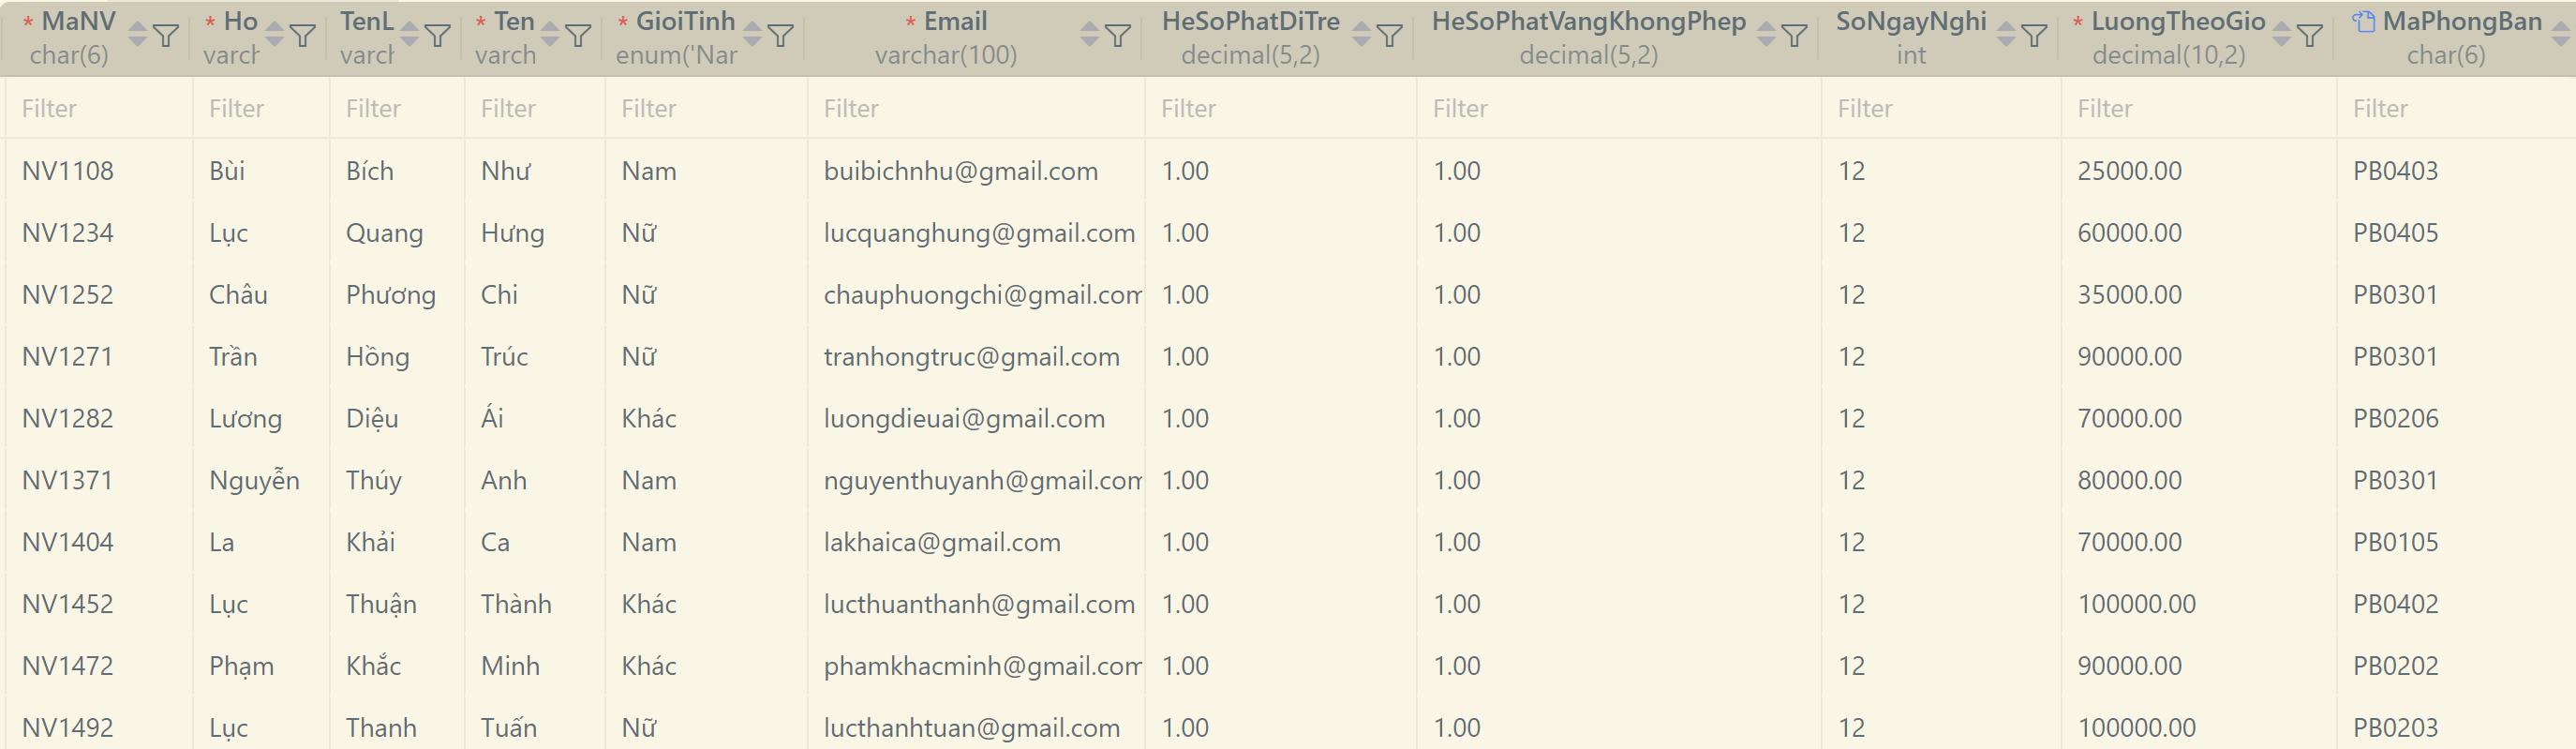
\includegraphics[width=\linewidth]{content/images/data_nhanvien.png}
        \caption{Dữ liệu bảng NhanVien}
        \label{fig:data_nhanvien}
    \end{figure}
\end{itemize}
\newpage
\subsubsection{Bảng Sdt\_NhanVien}
\begin{itemize}
    \item [--] Câu lệnh tạo bảng
   \begin{minted}{mysql}
CREATE TABLE Sdt_NhanVien (
    MaNV CHAR(6),
    SoDienThoai VARCHAR(10),
    PRIMARY KEY (MaNV, SoDienThoai),
    Foreign Key (MaNV) REFERENCES nhanvien(MaNV)
);
    \end{minted}
    \item [--] Câu lệnh ràng buộc
    \begin{minted}{mysql}
CREATE Trigger if NOT EXISTS checkSdtFormat 
BEFORE INSERT ON Sdt_NhanVien
FOR EACH ROW
BEGIN 
    IF (NOT EXISTS (SELECT 1 from nhanvien WHERE nhanvien.`MaNV`=NEW.MaNV)) THEN
        SIGNAL SQLSTATE '45000'
        SET MESSAGE_TEXT = 'Mã số nhân viên không tồn tại';
    END IF;

    IF NEW.SoDienThoai NOT REGEXP '^0[0-9]{9}' THEN
        SIGNAL SQLSTATE '45000'
        SET MESSAGE_TEXT = 'Số điện thoại phải bắt đầu bằng số 0 và có chính xác 10 chữ số';
    END IF;

    IF EXISTS (SELECT 1 from nhanvien NATURAL INNER JOIN Sdt_NhanVien WHERE `MaNV`=NEW.MaNV AND `SoDienThoai`=NEW.SoDienThoai) THEN
        SIGNAL SQLSTATE '45000'
        SET MESSAGE_TEXT = 'Nhân viên vừa nhập đã có số điện thoại trên';
    END IF;
END //
    \end{minted}
    \newpage
    \item [--] Câu lệnh thêm dữ liệu
   \begin{minted}{mysql}
INSERT INTO sdt_nhanvien 
VALUES 
    ('NV8058', '0649835291'),
    ('NV9750', '0429234781'),
    ('NV2034', '0111708152'),
    ('NV2790', '0720862287'),
    ('NV1452', '0819584592'),
    ('NV9714', '0688341035'),
    ('NV9858', '0235295264'),
    ('NV7733', '0437707384'),
    ('NV9240', '0248130737'),
    ('NV3993', '0290786034'),
    ...;
    \end{minted}
    \item [--] Kết quả dữ liệu của bảng
    \begin{figure}[H]
        \centering
        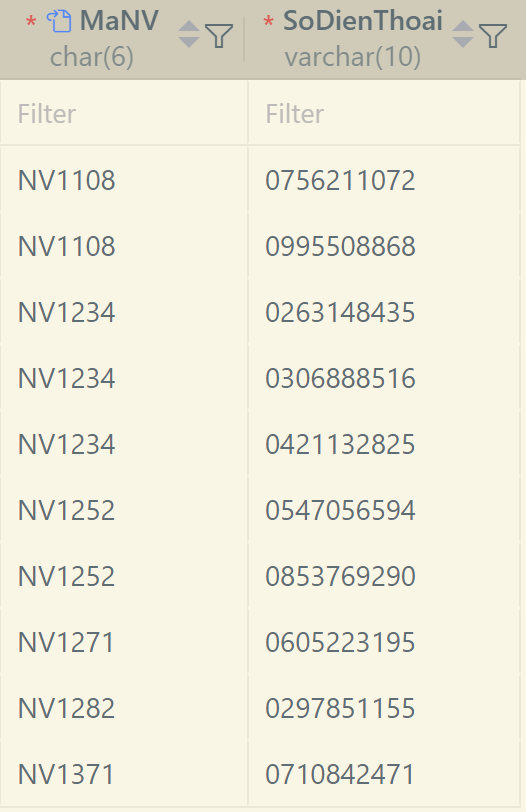
\includegraphics[width=0.5\linewidth]{content/images/data_sdtNV.png}
        \caption{Dữ liệu bảng Sdt\_NhanVien}
        \label{fig:data_sdtNV}
    \end{figure}
\end{itemize}
\newpage
\subsubsection{Bảng NhanVienToanThoiGian}
\begin{itemize}
    \item [--] Câu lệnh tạo bảng
    \begin{minted}{mysql}
CREATE TABLE NhanVienToanThoiGian (
    MaNV CHAR(6) PRIMARY KEY,
    GioBatDau TIME,
    GioKetThuc TIME,
    LuongTangCa DECIMAL(10, 2),
    MaNVQuanLy CHAR(6) DEFAULT NULL,
    FOREIGN KEY (MaNV) REFERENCES NhanVien(MaNV),
    Foreign Key (MaNVQuanLy) REFERENCES NhanVienToanThoiGian(MaNV)
);
    \end{minted}
    \item [--] Câu lệnh ràng buộc
    \begin{minted}{mysql}
-- Tối thêm sau
    \end{minted}
    \newpage
    \item [--] Câu lệnh thêm dữ liệu
    \begin{minted}{mysql}
INSERT INTO nhanvientoanthoigian(`MaNV`, `LuongTangCa`, `GioBatDau`, `GioKetThuc`)
VALUES
    ('NV1234', 90000.0, '08:00:00', '17:00:00'),
    ('NV1271', 135000.0, '08:00:00', '17:00:00'),
    ('NV1282', 105000.0, '08:00:00', '17:00:00'),
    ('NV1371', 120000.0, '08:00:00', '17:00:00'),
    ('NV1404', 105000.0, '08:00:00', '17:00:00'),
    ('NV1452', 150000.0, '08:00:00', '17:00:00'),
    ('NV1472', 135000.0, '08:00:00', '17:00:00'),
    ('NV1492', 150000.0, '08:00:00', '17:00:00'),
    ('NV1778', 135000.0, '08:00:00', '17:00:00'),
    ('NV1816', 75000.0, '08:00:00', '17:00:00'),
    ...;
    \end{minted}
    \item [--] Kết quả dữ liệu của bảng
    \begin{figure}[H]
        \centering
        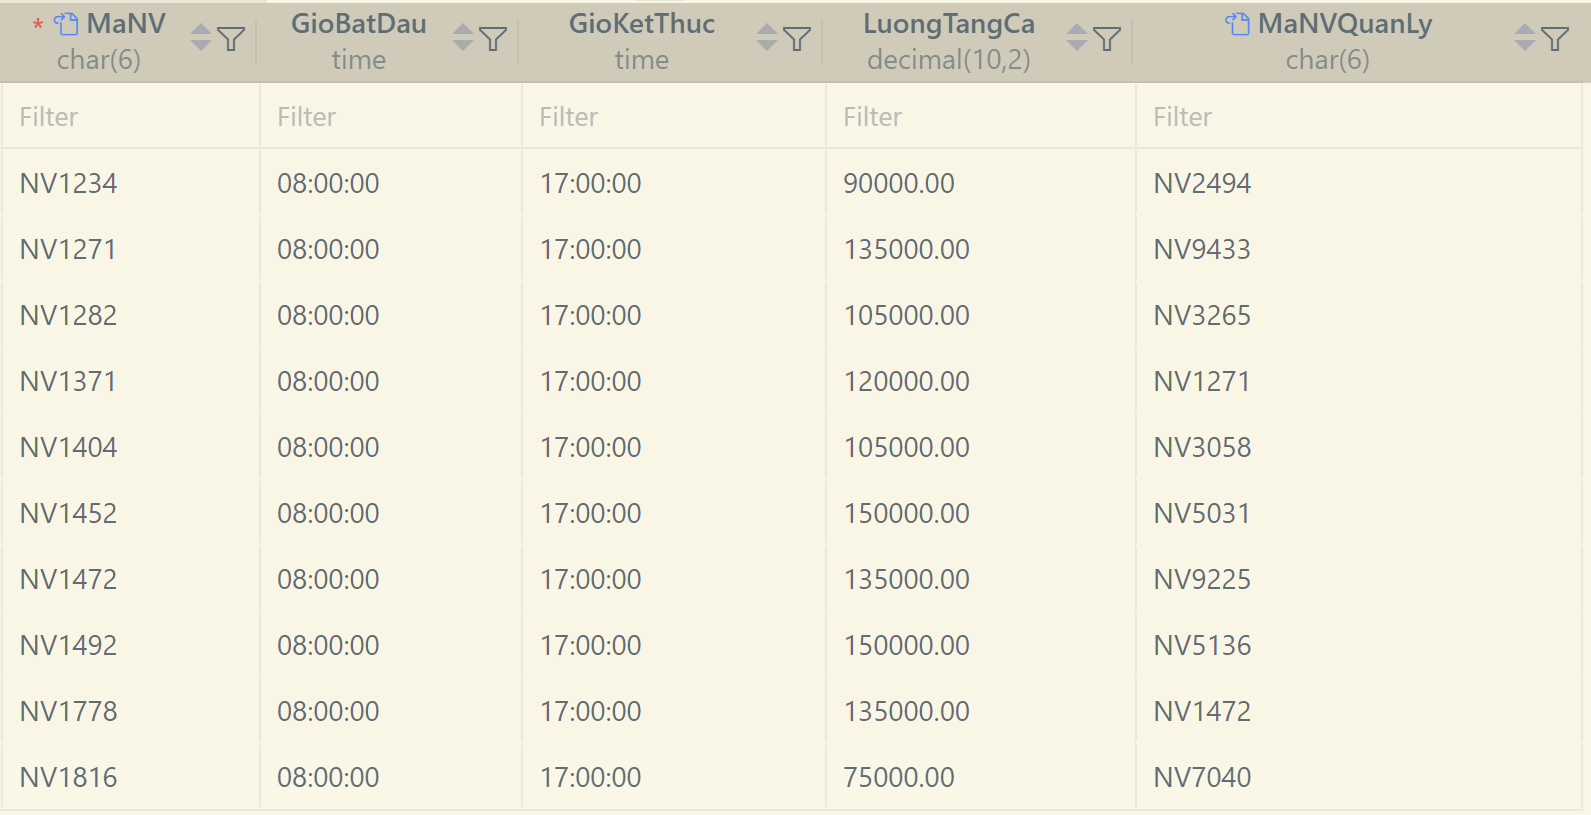
\includegraphics[width=\linewidth]{content/images/data_nvfulltime.png}
        \caption{Dữ liệu bảng NhanVienToanThoiGian}
        \label{fig:data_nvfulltime}
    \end{figure}
\end{itemize}
\newpage
\subsubsection{Bảng NhanVienBanThoiGian}
\begin{itemize}
    \item [--] Câu lệnh tạo bảng
   \begin{minted}{mysql}
CREATE TABLE NhanVienBanThoiGian (
    MaNV CHAR(6) PRIMARY KEY,
    MaNV_GiamSat CHAR(6),
    FOREIGN KEY (MaNV) REFERENCES NhanVien(MaNV),
    Foreign Key (MaNV_GiamSat) REFERENCES NhanVienToanThoiGian(MaNV)
);
    \end{minted}
    \item [--] Câu lệnh thêm dữ liệu
   \begin{minted}{mysql}
INSERT INTO nhanvienbanthoigian(`MaNV`, `MaNV_GiamSat`)
VALUES
    ('NV7733', 'NV9606'), ('NV8232', 'NV9606'),
    ('NV9199', 'NV9606'), ('NV8084', 'NV6786'),
    ('NV1540', 'NV4355'), ('NV8519', 'NV4355'),
    ('NV9375', 'NV1404'), ('NV3184', 'NV2357'),
    ('NV7938', 'NV2357'), ('NV9007', 'NV2357'),
    ...;
    \end{minted}
    \item [--] Kết quả dữ liệu của bảng
    \begin{figure}[H]
        \centering
        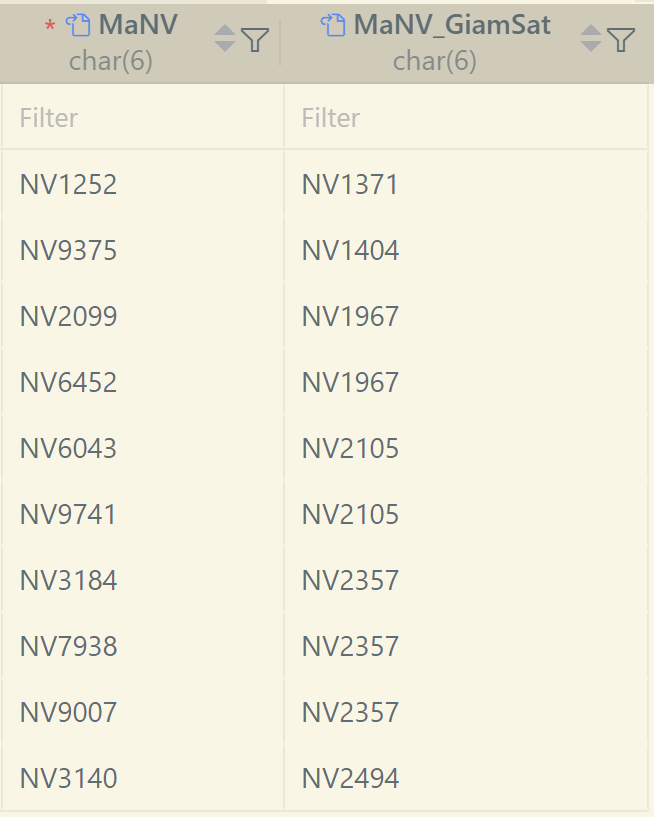
\includegraphics[width=0.45\linewidth]{content/images/data_nvparttime.png}
        \caption{Dữ liệu bảng NhanVienBanThoiGian}
        \label{fig:data_nvparttime}
    \end{figure}
\end{itemize}
\newpage
\subsubsection{Bảng DuAn}
\begin{itemize}
    \item [--] Câu lệnh tạo bảng
   \begin{minted}{mysql}
CREATE TABLE DuAn (
    MaDuAn CHAR(6) PRIMARY KEY,
    TenDuAn NVARCHAR(100) NOT NULL,
    MoTa TEXT,
    NgayBatDau DATE NOT NULL,
    NgayKetThuc DATE,
    Deadline DATE NOT NULL,
    MaPhongBan CHAR(6),
    MaQuanLy CHAR(6),
    FOREIGN KEY (MaPhongBan) REFERENCES PhongBan(MaPhongBan),
    FOREIGN KEY (MaQuanLy) REFERENCES NhanVienToanThoiGian(MaNV)
);
    \end{minted}
    \newpage
    \item [--] Câu lệnh ràng buộc
\begin{minted}{mysql}
CREATE TRIGGER checkDuAnFormat 
BEFORE INSERT ON DuAn
FOR EACH ROW
BEGIN
    IF NEW.MaDuAn NOT REGEXP '^DA[0-9]{4}$' THEN
        SIGNAL SQLSTATE '45000' 
        SET MESSAGE_TEXT = 'Mã dự án phải có định dạng DAxxxx, với 4 chữ số đằng sau';
    END IF;

    IF EXISTS (SELECT 1 from duan WHERE duan.MaDuAn=NEW.MaDuAn) THEN
        SIGNAL SQLSTATE '45000'
        SET MESSAGE_TEXT = 'Mã dự án đã tồn tại';
    END IF;

    IF NEW.TenDuAn NOT REGEXP '^[[:alnum:][:space:].,\\-]*$' THEN 
        SIGNAL SQLSTATE '45000'
        SET MESSAGE_TEXT = 'Tên dự án không được chứa ký tự đặc biệt';
    END IF;

    IF NEW.MoTa NOT REGEXP '^[[:alnum:][:space:][:punct:]]*$' THEN 
        SIGNAL SQLSTATE '45000'
        SET MESSAGE_TEXT = 'Mô tả không được chứa ký tự đặc biệt';
    END IF;

    IF (NOT EXISTS (SELECT 1 from nhanvien WHERE nhanvien.`MaNV`=NEW.MaQuanLy)) THEN
        SIGNAL SQLSTATE '45000'
        SET MESSAGE_TEXT = 'Mã số nhân viên quản lý dự án không tồn tại';
    END IF;

    IF (NOT EXISTS (SELECT 1 from phongban WHERE phongban.`MaPhongBan`=NEW.MaPhongBan)) THEN
        SIGNAL SQLSTATE '45000'
        SET MESSAGE_TEXT = 'Mã phòng ban không tồn tại';
    END IF;
END //
\end{minted}
    \newpage
    \item [--] Câu lệnh thêm dữ liệu
    \begin{minted}{mysql}
INSERT INTO duan(`MaDuAn`, `TenDuAn`, `MoTa`, `NgayBatDau`, `Deadline`, `NgayKetThuc`, `MaPhongBan`, `MaQuanLy`)
VALUES 
    ('DA0001', 'Theodore', 'Lorem ipsum d...t non varius.', '2023-12-01', '2024-01-08', '2024-01-05', 'PB0101', 'NV8120'),
    ('DA0002', 'Daphne', 'Sed arcu met...bus molestie.', '2024-01-10', '2024-01-25', NULL, 'PB0102', 'NV3058'),
    ('DA0003', 'Cora', 'Nulla plac...inibus.', '2024-02-10', '2024-03-13', '2024-03-13', 'PB0103', 'NV1816'),
    ('DA0004', 'Atticus', 'Praesent id m...nenatis.', '2024-03-15', '2024-03-23', '2024-03-23', 'PB0104', 'NV4036'),
    ('DA0005', 'Iris', 'Curabit...lectus.', '2024-03-20', '2024-04-15', '2024-04-15', 'PB0105', 'NV1404'),
    ('DA0006', 'Atlas', 'Vivamu...lla egestas dignissim.', '2024-03-21', '2024-04-23', '2024-04-23', 'PB0106', 'NV2357'),
    ('DA0007', 'Phoebe', 'Aenean nunc ...in semper nisl.', '2024-04-23', '2024-04-30', '2024-04-28', 'PB0201', 'NV9225'),
    ('DA0008', 'Ophelia', 'Curabi...dictum tortor.', '2024-04-30', '2024-05-16', '2024-05-10', 'PB0202', 'NV1472'),
    ('DA0009', 'Elias', 'Cras tempor ma...alesuada fames ac turpis egestas.', '2024-05-10', '2024-06-05', '2024-06-05', 'PB0203', 'NV1492'),
    ('DA0010', 'Zephyr', 'Integer ne...ces suscipit.', '2024-05-13', '2024-06-23', '2024-06-23', 'PB0204', 'NV3795'),
    ...;
    \end{minted}
    \item [--] Kết quả dữ liệu của bảng
    \begin{figure}[H]
        \centering
        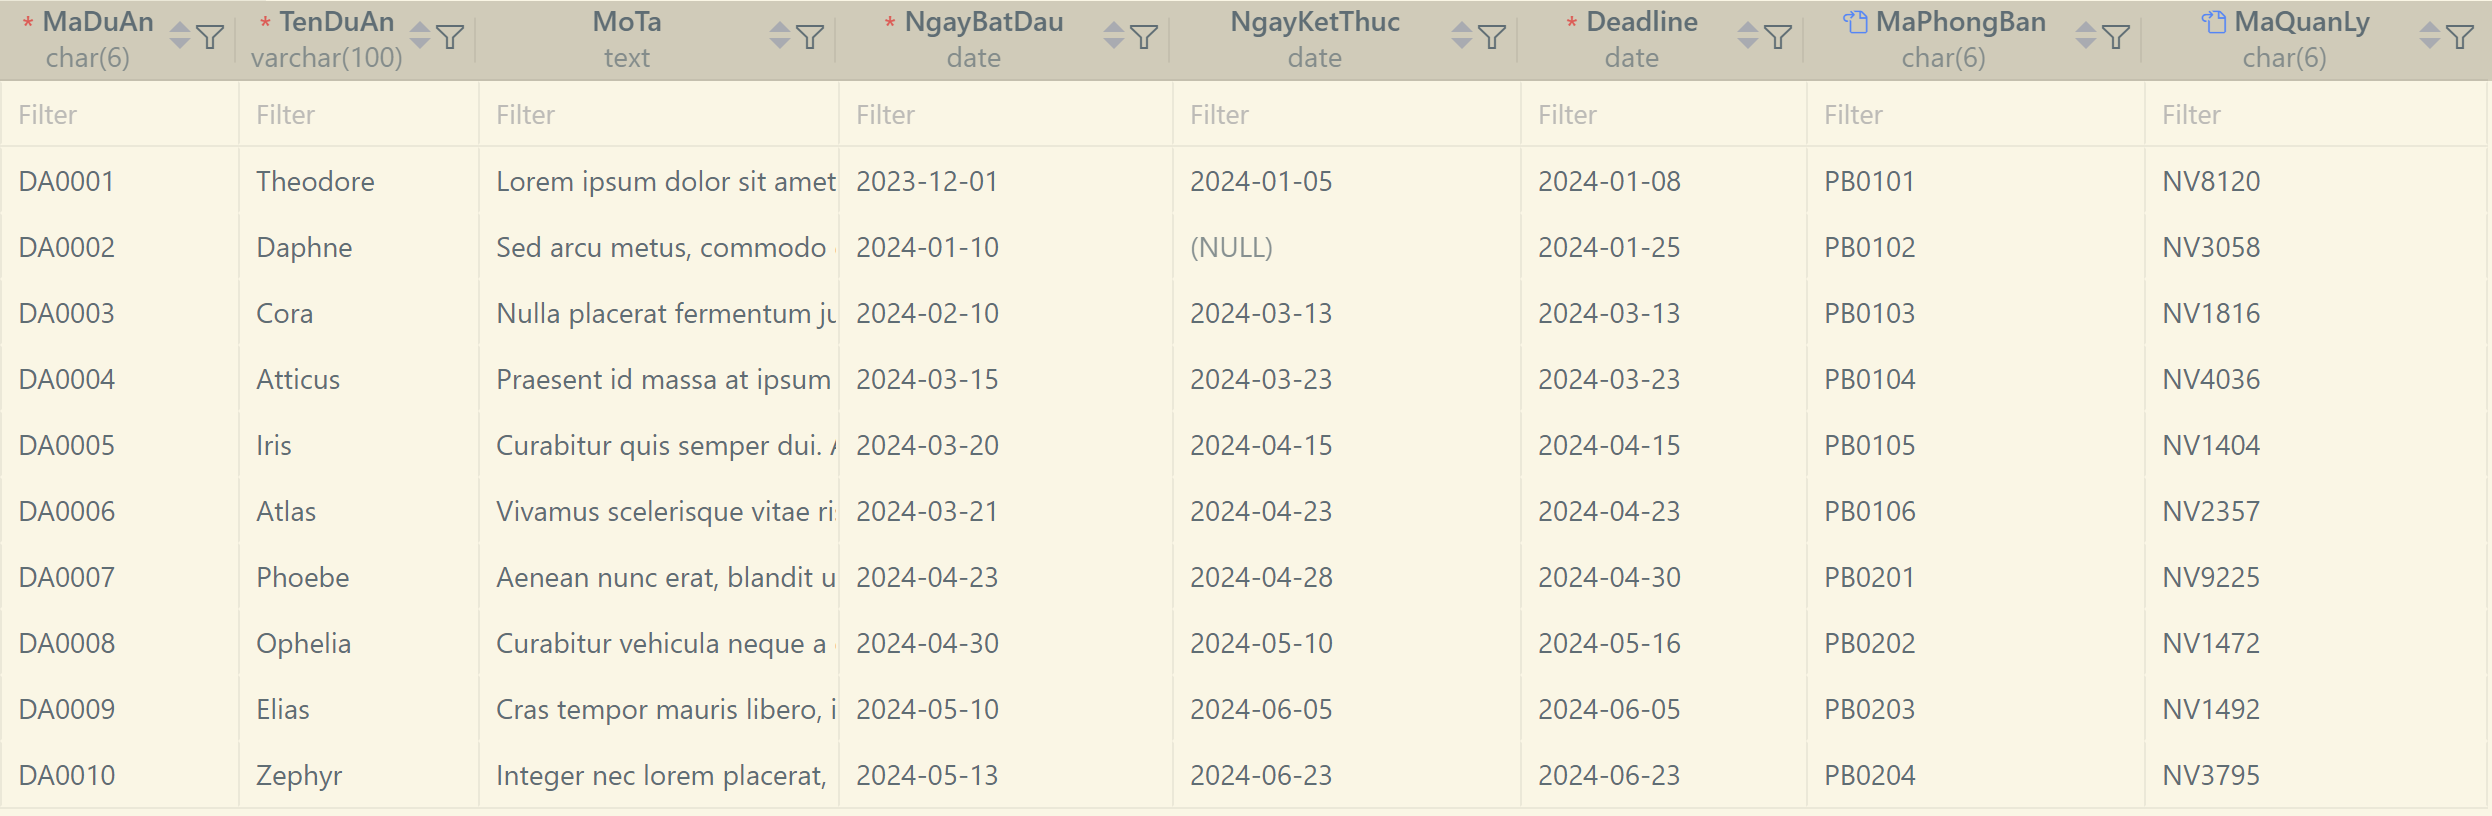
\includegraphics[width=1\linewidth]{content/images/data_duan.png}
        \caption{Dữ liệu của bảng DuAn}
        \label{fig:data_duan}
    \end{figure}
\end{itemize}
\subsubsection{Bảng NhanVienThamGiaDuAn}
\begin{itemize}
    \item [--] Câu lệnh tạo bảng
    \begin{minted}{mysql}
CREATE TABLE NhanVienThamGiaDuAn (
    MaNhanVien CHAR(6),
    MaDuAn CHAR(6),
    PRIMARY KEY (MaNhanVien, MaDuAn),
    Foreign Key (MaNhanVien) REFERENCES NhanVien(MaNV),
    Foreign Key (MaDuAn) REFERENCES DuAn(MaDuAn)
);
    \end{minted}
    \item [--] Câu lệnh ràng buộc
    \begin{minted}{mysql}
CREATE TRIGGER checkNhanVienThamGiaDuAnFormat 
BEFORE INSERT ON NhanVienThamGiaDuAn
FOR EACH ROW
BEGIN
    IF (NOT EXISTS (SELECT 1 from nhanvien WHERE nhanvien.`MaNV`=NEW.MaNhanVien)) THEN
        SIGNAL SQLSTATE '45000'
        SET MESSAGE_TEXT = 'Mã số nhân viên không tồn tại';
    END IF;

    IF (NOT EXISTS (SELECT 1 from DuAn WHERE DuAn.`MaDuAn`=NEW.MaDuAn)) THEN
        SIGNAL SQLSTATE '45000'
        SET MESSAGE_TEXT = 'Mã số dự án không tồn tại';
    END IF;

    IF EXISTS (SELECT 1 FROM NhanVienThamGiaDuAn WHERE NhanVienThamGiaDuAn.`MaNhanVien`=NEW.`MaNhanVien` AND NhanVienThamGiaDuAn.`MaDuAn`=NEW.`MaDuAn`) THEN
        SIGNAL SQLSTATE '45000'
        SET MESSAGE_TEXT = 'Nhân viên vừa nhập đã tham gia dự án trên';
    END IF;
END //
    \end{minted}
    \newpage
    \item [--] Câu lệnh thêm dữ liệu
   \begin{minted}{mysql}

INSERT INTO nhanvienthamgiaduan(`MaDuAn`, `MaNhanVien`)
VALUES
    ('DA0001', 'NV8120'),
    ('DA0002', 'NV3058'),
    ('DA0003', 'NV1816'),
    ('DA0004', 'NV4036'),
    ('DA0005', 'NV1404'),
    ('DA0006', 'NV2357'),
    ('DA0007', 'NV9225'),
    ('DA0008', 'NV1472'),
    ('DA0009', 'NV1492'),
    ('DA0010', 'NV3795'),
    ('DA0011', 'NV9750'),
    ('DA0012', 'NV7288'),
    ...;
    \end{minted}
    \item [--] Kết quả dữ liệu của bảng
    \begin{figure}[H]
        \centering
        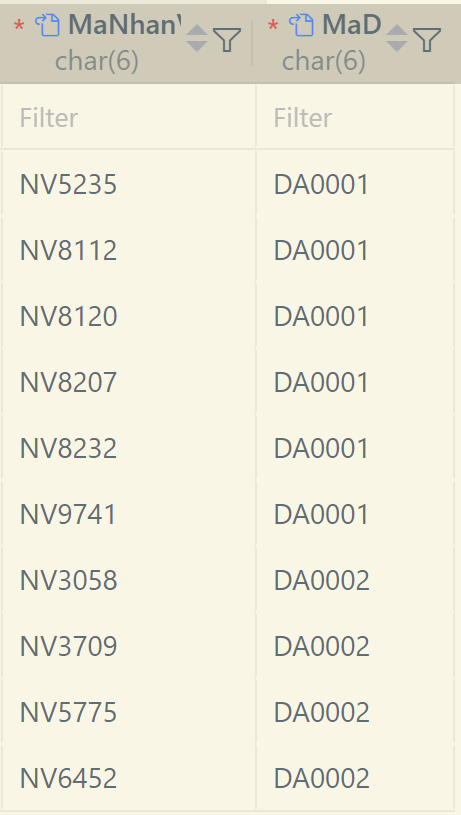
\includegraphics[width=0.4\linewidth]{content/images/data_nhanvien_duan.png}
        \caption{Dữ liệu của bảng NhanVienThamGiaDuAn} 
        \label{fig:data_nhanvien_duan}
    \end{figure}
\end{itemize}
\newpage
\subsubsection{Bảng NguoiPhuThuoc}
\begin{itemize}
    \item [--] Câu lệnh tạo bảng
   \begin{minted}{mysql}
CREATE TABLE NguoiPhuThuoc (
    Ten NVARCHAR(50),
    GioiTinh ENUM('Nam', 'Nữ', 'Khác') NOT NULL,
    SoDienThoai VARCHAR(10) NOT NULL,
    MoiQuanHe NVARCHAR(50) NOT NULL,
    MaNV CHAR(6),
    PRIMARY KEY (Ten, MaNV),
    FOREIGN KEY (MaNV) REFERENCES NhanVien(MaNV)
);
    \end{minted}
    \newpage
    \item [--] Câu lệnh ràng buộc
    \begin{minted}{mysql}
CREATE TRIGGER IF NOT EXISTS checkNguoiPhuThuocFormat
BEFORE INSERT on NguoiPhuThuoc
FOR EACH ROW
BEGIN
    IF NEW.Ten NOT REGEXP '^[[:alnum:][:space:]]*$' THEN 
        SIGNAL SQLSTATE '45000'
        SET MESSAGE_TEXT = 'Tên người phụ thuộc không được chứa những ký tự đặc biệt';
    END IF;

    IF NEW.MoiQuanHe NOT REGEXP '^[[:alnum:][:space:]]*$' THEN 
        SIGNAL SQLSTATE '45000'
        SET MESSAGE_TEXT = 'Tên mối quan hệ không được chứa những ký tự đặc biệt';
    END IF;

    IF NEW.SoDienThoai NOT REGEXP '^0[0-9]{9}' THEN
        SIGNAL SQLSTATE '45000'
        SET MESSAGE_TEXT = 'Số điện thoại phải bắt đầu bằng số 0 và có chính xác 10 chữ số';
    END IF;

    IF (NOT EXISTS (SELECT 1 from nhanvien WHERE nhanvien.`MaNV`=NEW.MaNV)) THEN
        SIGNAL SQLSTATE '45000'
        SET MESSAGE_TEXT = 'Mã số nhân viên không tồn tại';
    END IF;
END//
    \end{minted}
    \newpage
    \item [--] Câu lệnh thêm dữ liệu
    \begin{minted}{mysql}
INSERT INTO nguoiphuthuoc(`MaNV`, `Ten`, `SoDienThoai`, `GioiTinh`, `MoiQuanHe`)
VALUES
    ('NV7733', 'Nguyễn Thị Mỷ Ngọc', '0318269338', 'Nữ', 'Chồng'),
    ('NV8120', 'Nguyễn Lê Hoài Ân', '0891190428', 'Nữ', 'Cha'),
    ('NV8232', 'Nguyễn Như Mười', '0452543489', 'Nữ', 'Cha'),
    ('NV9199', 'Lê Anh Hải', '0796135045', 'Nữ', 'Mẹ'),
    ('NV9606', 'Huỳnh Hữu Thoại', '0164997442', 'Nam', 'Con'),
    ('NV3058', 'Mai Trúc Anh', '0341137858', 'Nữ', 'Chồng'),
    ('NV3189', 'Ngô Minh Mẫn', '0839219566', 'Nữ', 'Vợ'),
    ('NV3308', 'Lê Quyết Tiến', '0229990080', 'Nữ', 'Mẹ'),
    ('NV3577', 'Nguyễn Văn Dũng', '0130696033', 'Nữ', 'Vợ'),
    ('NV4286', 'Trần Công Danh', '0464749368', 'Nam', 'Chồng'),
    ...;
    \end{minted}
    \item [--] Kết quả dữ liệu của bảng
    \begin{figure}[H]
        \centering
        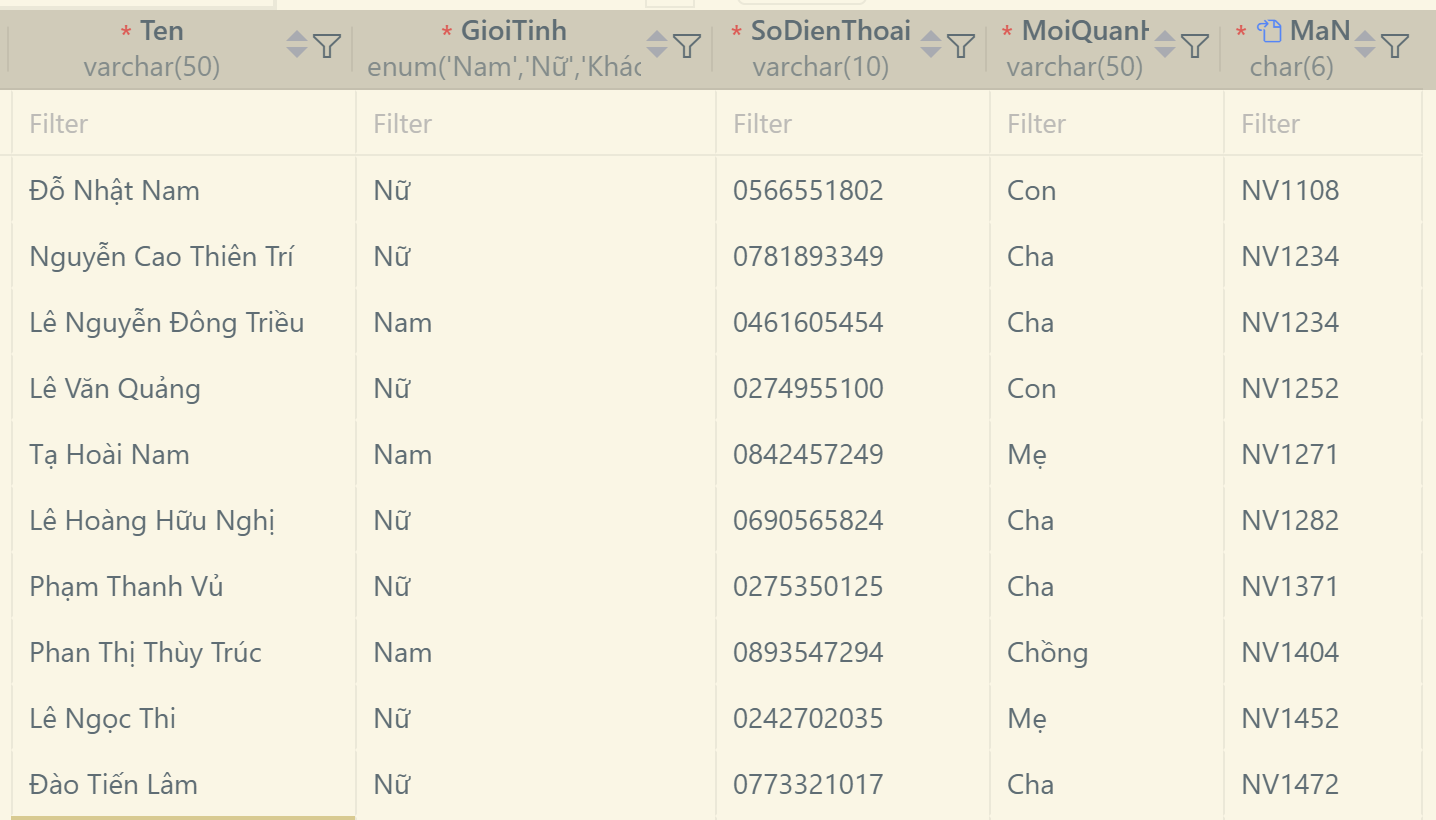
\includegraphics[width=1\linewidth]{content/images/data_nguoiphuthuoc.png}
        \caption{Dữ liệu của bảng NguoiPhuThuoc}
        \label{fig:data_nguoiphuthuoc}
    \end{figure}
\end{itemize}
\newpage
\subsubsection{Bảng BangChamCong}
\begin{itemize}
    \item [--] Câu lệnh tạo bảng
   \begin{minted}{mysql}
CREATE TABLE BangChamCong (
    MaNV CHAR(6),
    Ngay DATE,
    TrangThai ENUM('Có mặt', 'Vắng có phép', 'Vắng không phép'),
    TongSoGioLam DECIMAL(5, 2) DEFAULT 0,
    PRIMARY KEY (MaNV, Ngay),
    FOREIGN KEY (MaNV) REFERENCES NhanVien(MaNV)
);
    \end{minted}
    \item [--] Câu lệnh ràng buộc
   \begin{minted}{mysql}
CREATE TRIGGER checkBangChamCongFormat 
BEFORE INSERT ON BangChamCong
FOR EACH ROW
BEGIN
    IF (NOT EXISTS (SELECT 1 from nhanvien WHERE nhanvien.`MaNV`=NEW.MaNV)) THEN
        SIGNAL SQLSTATE '45000'
        SET MESSAGE_TEXT = 'Mã số nhân viên không tồn tại';
    END IF;
END //
    \end{minted}
    \newpage
    \item [--] Câu lệnh thêm dữ liệu
   \begin{minted}{mysql}
INSERT INTO bangchamcong(`MaNV`, `Ngay`, `TrangThai`)
VALUES
    ('NV1234', '2024-10-21', 'Có mặt'),
    ('NV1234', '2024-10-22', 'Có mặt'),
    ('NV1234', '2024-10-23', 'Có mặt'),
    ('NV1234', '2024-10-24', 'Có mặt'),
    ('NV1234', '2024-10-25', 'Có mặt'),
    ('NV1234', '2024-10-28', 'Có mặt'),
    ('NV1234', '2024-10-29', 'Vắng không phép'),
    ('NV1234', '2024-10-30', 'Vắng không phép'),
    ('NV1234', '2024-10-31', 'Có mặt'),
    ('NV1234', '2024-11-01', 'Có mặt'),
    ...;
    \end{minted}
    \item [--] Kết quả dữ liệu của bảng
    \begin{figure}[H]
        \centering
        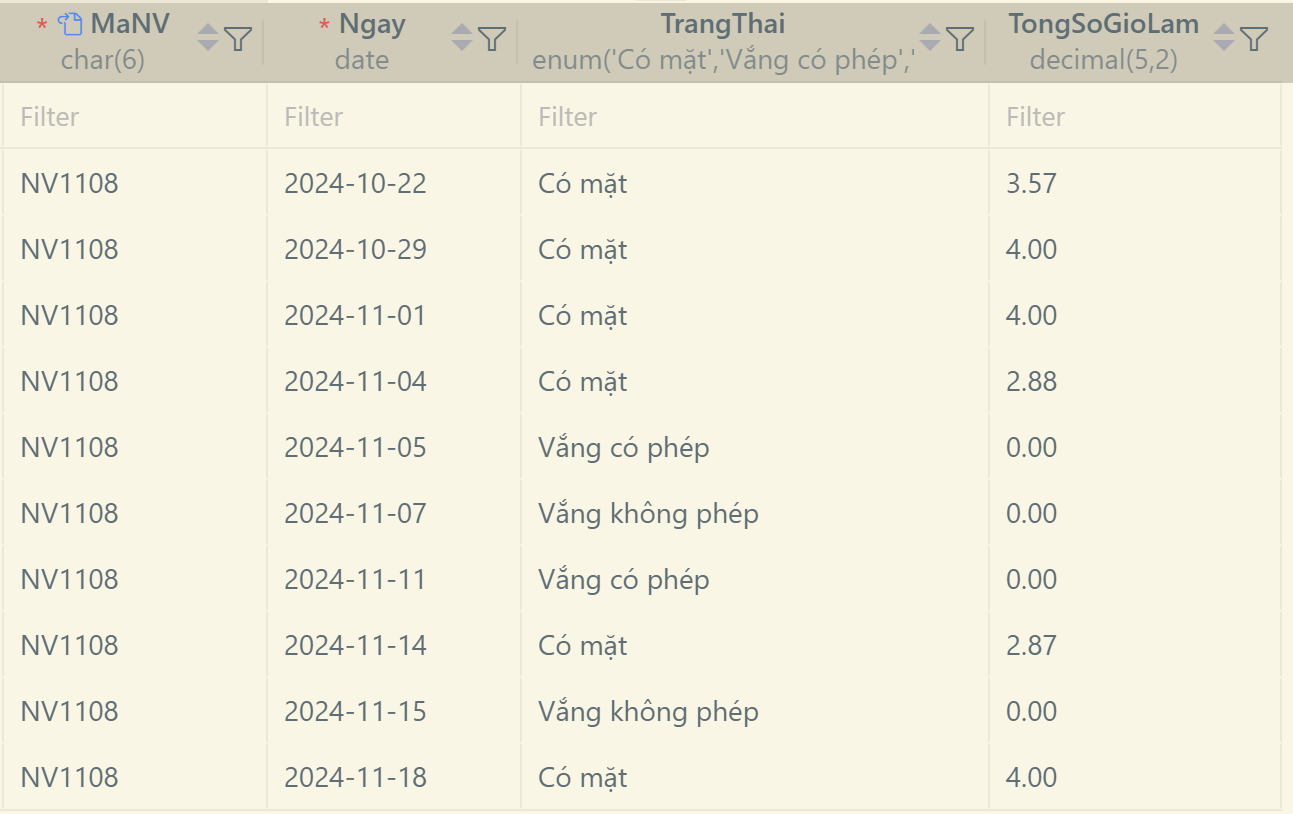
\includegraphics[width=\linewidth]{content/images/data_bangchamcong.png}
        \caption{Dữ liệu của bảng BangChamCong}
        \label{fig:data_bangchamcong}
    \end{figure}
\end{itemize}
\newpage
\subsubsection{Bảng LanRaVao}
\begin{itemize}
    \item [--] Câu lệnh tạo bảng
   \begin{minted}{mysql}
CREATE TABLE LanRaVao (
    MaNV CHAR(6),
    Ngay DATE,
    GioVao TIME,
    GioRa TIME,
    PRIMARY KEY (MaNV, Ngay, GioVao, GioRa),
    FOREIGN KEY (MaNV, Ngay) REFERENCES BangChamCong(MaNV, Ngay)
);
    \end{minted}
    \item [--] Câu lệnh ràng buộc
   \begin{minted}{mysql}
CREATE TRIGGER checkLanRaVaoFormat 
BEFORE INSERT ON LanRaVao
FOR EACH ROW
BEGIN
    IF (NOT EXISTS (SELECT 1 from nhanvien WHERE nhanvien.`MaNV`=NEW.MaNV)) THEN
        SIGNAL SQLSTATE '45000'
        SET MESSAGE_TEXT = 'Mã số nhân viên không tồn tại';
    END IF;
END //
    \end{minted}
    \newpage
    \item [--] Câu lệnh thêm dữ liệu
   \begin{minted}{mysql}
INSERT INTO lanravao (`MaNV`, `Ngay`, `GioVao`, `GioRa`) 
VALUES
    ('NV1234', '2024-10-21', '08:00', '12:00'),
    ('NV1234', '2024-10-21', '13:00', '17:00'),
    ('NV1234', '2024-10-22', '08:00', '12:00'),
    ('NV1234', '2024-10-22', '13:00', '17:00'),
    ('NV1234', '2024-10-23', '08:18', '12:00'),
    ('NV1234', '2024-10-23', '13:00', '17:00'),
    ('NV1234', '2024-10-24', '08:00', '11:07'),
    ('NV1234', '2024-10-24', '13:00', '17:00'),
    ('NV1234', '2024-10-25', '08:00', '12:00'),
    ('NV1234', '2024-10-25', '13:00', '17:00'),
    ...;
    \end{minted}
    \item [--] Kết quả dữ liệu của bảng
    \begin{figure}[H]
        \centering
        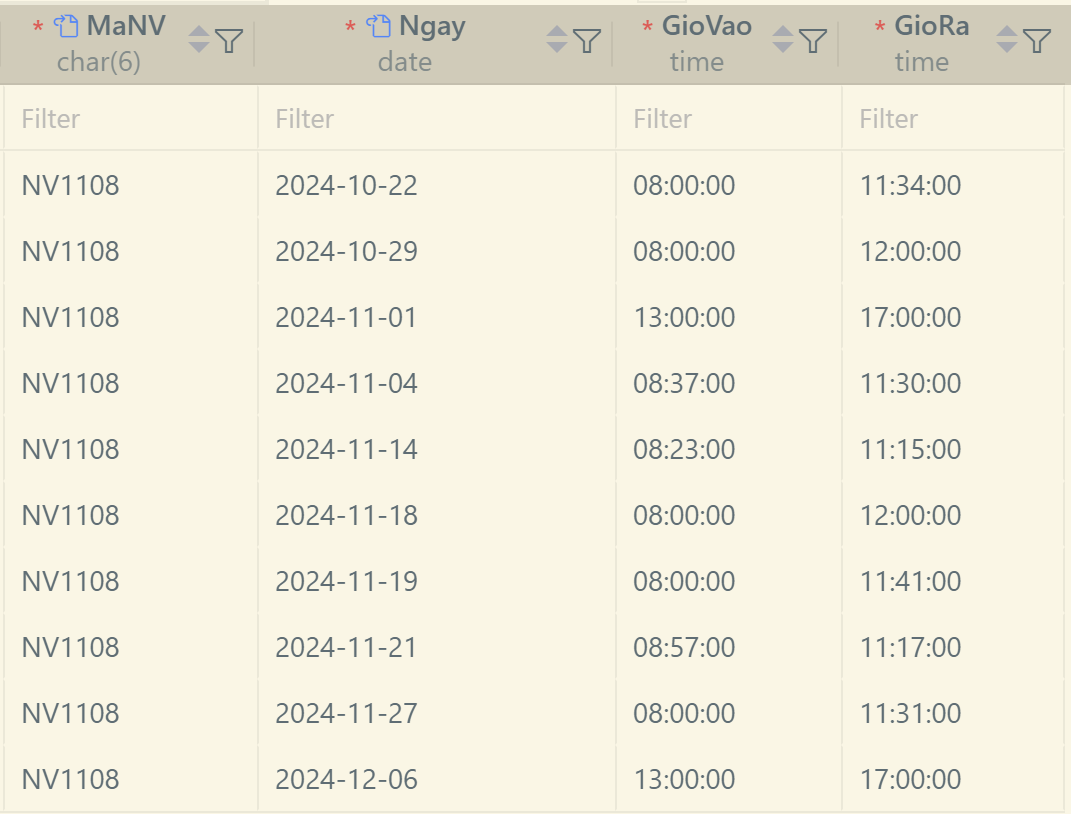
\includegraphics[width=1\linewidth]{content/images/data_lanravao.png}
        \caption{Dữ liệu của bảng LanRaVao}
        \label{fig:data_lanravao}
    \end{figure}
\end{itemize}
\newpage
\subsubsection{Bảng LichLamViec}
\begin{itemize}
    \item [--] Câu lệnh tạo bảng
   \begin{minted}{mysql}
CREATE TABLE LichLamViec (
    MaNV CHAR(6),
    Ngay DATE,
    GioBatDau TIME,
    GioKetThuc TIME,
    PRIMARY KEY (MaNV, Ngay, GioBatDau, GioKetThuc),
    FOREIGN KEY (MaNV) REFERENCES NhanVienBanThoiGian(MaNV)
);
    \end{minted}
    \item [--] Câu lệnh ràng buộc
   \begin{minted}{mysql}
CREATE TRIGGER checkLichLamViecFormat 
BEFORE INSERT ON LichLamViec
FOR EACH ROW
BEGIN
    IF (NOT EXISTS (SELECT 1 from nhanvien WHERE nhanvien.`MaNV`=NEW.MaNV)) THEN
        SIGNAL SQLSTATE '45000'
        SET MESSAGE_TEXT = 'Mã số nhân viên không tồn tại';
    END IF;
END //
    \end{minted}
    \newpage
    \item [--] Câu lệnh thêm dữ liệu
   \begin{minted}{mysql}
INSERT INTO lichlamviec(`MaNV`, `Ngay`, `GioBatDau`, `GioKetThuc`)
VALUES
    ('NV1252', '2024-10-21', '08:00', '12:00'),
    ('NV1252', '2024-10-23', '13:00', '17:00'),
    ('NV1252', '2024-10-24', '13:00', '17:00'),
    ('NV1252', '2024-10-29', '08:00', '12:00'),
    ('NV1252', '2024-11-01', '13:00', '17:00'),
    ('NV1252', '2024-11-04', '08:00', '12:00'),
    ('NV1252', '2024-11-06', '13:00', '17:00'),
    ('NV1252', '2024-11-08', '08:00', '12:00'),
    ('NV1252', '2024-11-12', '13:00', '17:00'),
    ('NV1252', '2024-11-15', '08:00', '12:00'),
    ...;
    \end{minted}
    \item [--] Kết quả dữ liệu của bảng
    \begin{figure}[H]
        \centering
        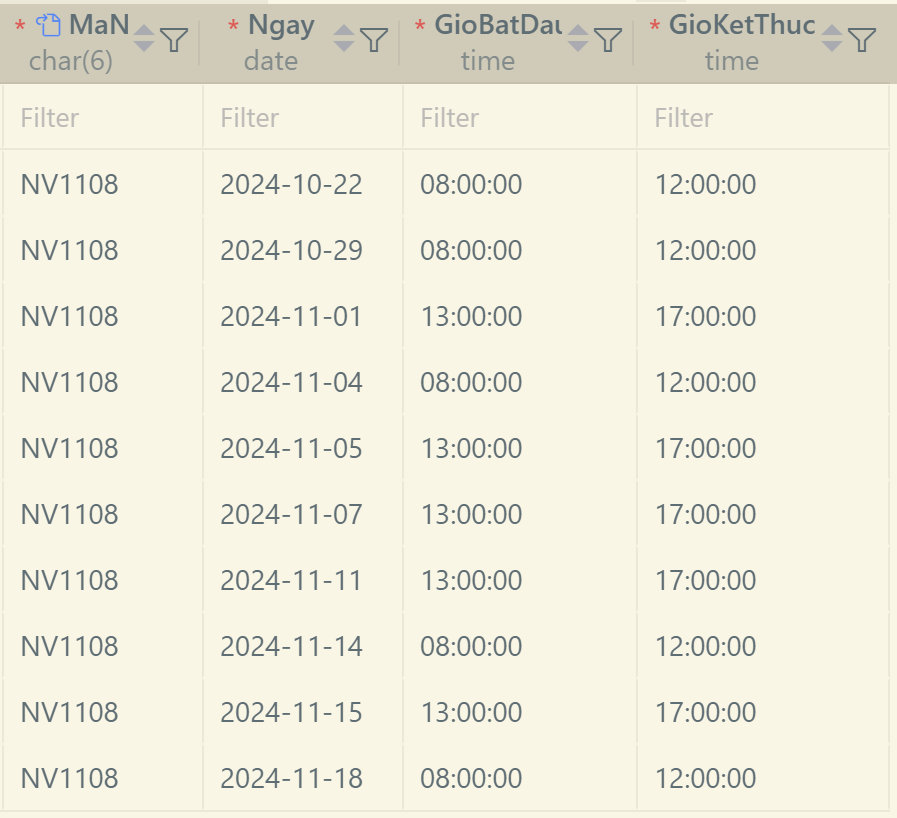
\includegraphics[width=0.9\linewidth]{content/images/data_lichlamviec.png}
        \caption{Dữ liệu của bảng LichLamViec}
        \label{fig:data_lichlamviec}
    \end{figure}
\end{itemize}
\newpage
\subsubsection{Bảng BangThietLapLuong}
\begin{itemize}
    \item [--] Câu lệnh tạo bảng
   \begin{minted}{mysql}
CREATE TABLE BangThietLapLuong (
    NgayApDung DATE PRIMARY KEY,
    ThueSuat DECIMAL(5, 2),
    BaoHiemXH DECIMAL(5, 2)
);
    \end{minted}
    \item [--] Câu lệnh thêm dữ liệu
   \begin{minted}{mysql}
INSERT INTO bangthietlapluong(`NgayApDung`, `ThueSuat`, `BaoHiemXH`) 
VALUES  
    ('2024-10-01', 0.10, 0.08),
    ('2024-11-25', 0.08, 0.08);
    \end{minted}
    \item [--] Kết quả dữ liệu của bảng
    \begin{figure}[H]
        \centering
        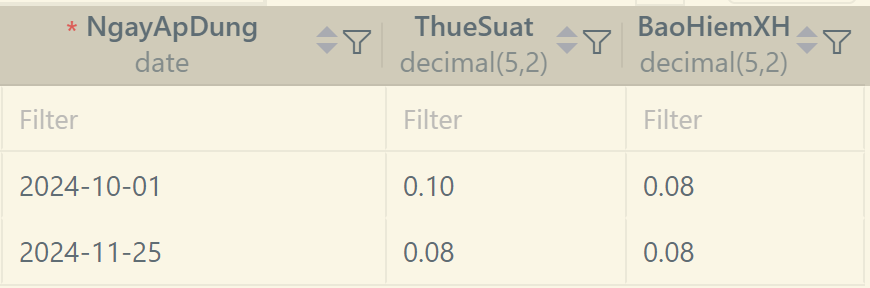
\includegraphics[width=1\linewidth]{content/images/data_bangthietlap.png}
        \caption{Dữ liệu của bảng BangThietLapLuong}
        \label{fig:data_bangthietlap}
    \end{figure}
\end{itemize}
\newpage
\subsubsection{Bảng BangLuong}
\begin{itemize}
    \item [--] Câu lệnh tạo bảng
   \begin{minted}{mysql}
CREATE TABLE BangLuong (
    MaNV CHAR(6),
    NgayBatDau DATE,
    NgayKetThuc DATE,
    NgayApDung DATE,
    PRIMARY KEY (MaNV, NgayBatDau, NgayKetThuc),
    FOREIGN KEY (MaNV) REFERENCES NhanVien(MaNV),
    FOREIGN KEY (NgayApDung) REFERENCES BangThietLapLuong(NgayApDung)
);
    \end{minted}
    \item [--] Câu lệnh ràng buộc
   \begin{minted}{mysql}
CREATE TRIGGER checkBangLuongFormat 
BEFORE INSERT ON BangLuong
FOR EACH ROW
BEGIN
    IF (NOT EXISTS (SELECT 1 from nhanvien WHERE nhanvien.`MaNV`=NEW.MaNV)) THEN
        SIGNAL SQLSTATE '45000'
        SET MESSAGE_TEXT = 'Mã số nhân viên không tồn tại';
    END IF;
END //
    \end{minted}
    \newpage
    \item [--] Câu lệnh thêm dữ liệu
   \begin{minted}{mysql}
INSERT INTO bangluong(`MaNV`, `NgayBatDau`, `NgayKetThuc`, `NgayApDung`) 
VALUES
    ('NV1108', '2024-10-21', '2024-10-31', '2024-10-01'),
    ('NV1108', '2024-11-01', '2024-11-30', '2024-11-25'),
    ('NV1234', '2024-10-21', '2024-10-31', '2024-10-01'),
    ('NV1234', '2024-11-01', '2024-11-30', '2024-11-25'),
    ('NV1252', '2024-10-21', '2024-10-31', '2024-10-01'),
    ('NV1252', '2024-11-01', '2024-11-30', '2024-11-25'),
    ('NV1271', '2024-10-21', '2024-10-31', '2024-10-01'),
    ('NV1271', '2024-11-01', '2024-11-30', '2024-11-25'),
    ('NV1282', '2024-10-21', '2024-10-31', '2024-10-01'),
    ('NV1282', '2024-11-01', '2024-11-30', '2024-11-25'),
    ...;
    \end{minted}
    \item [--] Kết quả dữ liệu của bảng
    \begin{figure}[H]
        \centering
        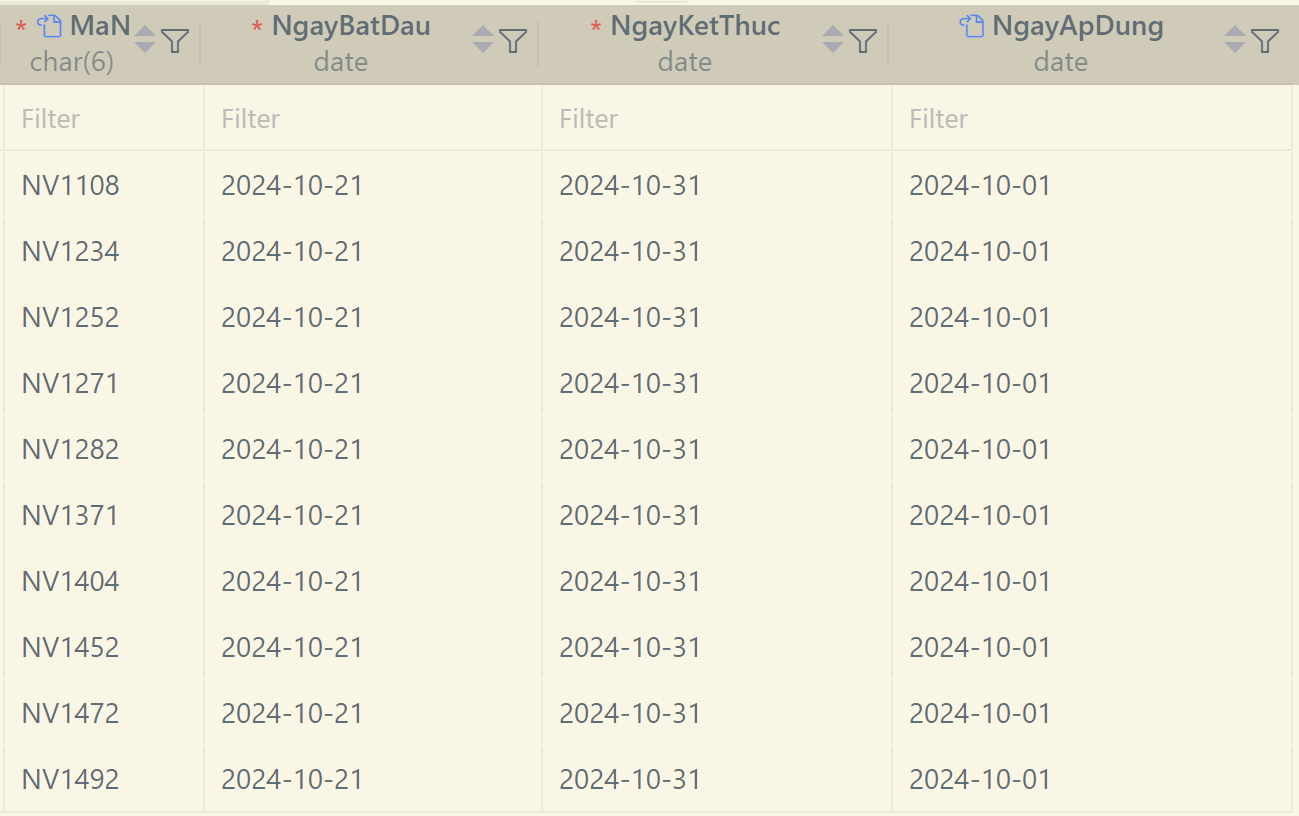
\includegraphics[width=1\linewidth]{content/images/data_bangluong.png}
        \caption{Dữ liệu của bảng BangLuong}
        \label{fig:data_bangluong}
    \end{figure}
\end{itemize}



\newpage